\documentclass[11pt]{article}
\usepackage{icmlko}
\begin{document}

\title{잘게는 좋고 넓게는 나쁘다 --- 하루 만에 내 설명을 물린다}
\author{월드모델 실험실}
\date{노트 421 · 2026년 8월 2일}
\maketitle

\begin{abstract}
노트 420이 두 번째 도메인 표지를 물리면서 이유를 이렇게 적었다 ---
\emph{둘째부터는 학습 도메인 집합을 더 잘게 깎는 데 쓰이고, 그렇게 깎을수록
모형이 그 열한 개에 맞춰진다.} 그 설명이 맞으면 \textbf{표지 하나 안에서도}
같은 일이 나야 한다: 갈래를 잘게 할수록 전이가 나빠져야 한다.

쟀다. 덮음을 고정한 채 --- 위 $K$ 무리만 이름을 두고 나머지는 ``기타'' 한
무리로 묶어 --- 갈래 수만 줄였다.

\begin{center}
\begin{tabular}{lrrr}
\hline
$K$ & 칸 수 & 판 & KR 만화 전이 \\
\hline
2 & 18 & $+0.4707$ & $+0.0788$ \\
3 & 21 & $+0.4677$ & $+0.1502$ \\
5 & 25 & $+0.4692$ & $+0.0955$ \\
\textbf{전부} & \textbf{40} & $\mathbf{+0.4723}$ & $\mathbf{+0.1946}$ \\
\hline
\end{tabular}
\end{center}

\textbf{반대로 나왔다.} 잘게 할수록 전이가 \emph{좋다}. 같은 유보 행 짝
되뽑기로 확인했다 --- 전부 $-$ $K{=}3$ 은 $+0.0493$ 95\%
$[+0.0100, +0.0919]$($0.999$), 전부 $-$ $K{=}2$ 는 $+0.1138$ 95\%
$[+0.0718, +0.1651]$($1.000$). \textbf{둘 다 확실하다.}

\textbf{그러므로 노트 420의 설명은 틀렸다.} 하루 만에 물린다.
\end{abstract}

\section{두 조작은 다른 일이다}

이제 둘이 나란히 놓인다. 같은 자로 잰 전이 변화다.

\begin{center}
\begin{tabular}{lrl}
\hline
조작 & 전이 변화 & \\
\hline
표지 하나를 \textbf{잘게} ($K{=}2 \to$ 전부) & $\mathbf{+0.1138}$ & $[+0.072, +0.165]$ \\
표지를 \textbf{하나 더} (grp $\to$ grp$+$grp2) & $\mathbf{-0.1140}$ & $[-0.159, -0.067]$ \\
\hline
\end{tabular}
\end{center}

크기가 거의 같고 부호가 반대다. \textbf{``칸을 늘린다''로는 둘을 같이 못
설명한다} --- 둘 다 칸을 늘리는데 하나는 사고 하나는 판다.

\section{고쳐 적는 설명}

표지 \textbf{하나}일 때, 그 열의 눈금은 \textbf{도메인 사이에서 공유된다}
--- $0.0$ 은 어느 도메인에서나 ``이 도메인의 제일 큰 무리''를 뜻한다.
갈래를 잘게 해도 그 성질은 그대로다. 나무가 그 열로 가르면 열한 도메인을
\emph{한꺼번에} 가르는 규칙이 된다. 잘수록 그 규칙이 정교해지니 좋다.

표지가 \textbf{둘}이면 나무가 둘을 \textbf{곱해서} 쓸 수 있다.
(표지1 $\times$ 표지2)의 칸은 도메인을 \textbf{콕 집는} 데 쓰기 좋고 ---
예컨대 ``\texttt{source}$=$manga 이고 \texttt{age\_type}$=$전체가''는
사실상 한 도메인이다 --- 그러면 원핫이 하던 일을 되살리는 셈이다.
\textbf{해로운 것은 칸 수가 아니라 곱이다.}

이 읽기는 노트 404와도 맞는다 --- 관측 표시자 무늬만으로 열한 중 아홉이
순도 $1.000$ 이었다. \textbf{도메인을 콕 집는 길은 이미 넘친다}; 하나 더
내는 것이 값이 아니다.

\section{남은 것}

\begin{tabular}{lp{7.0cm}}
\hline
곱을 막고 표지는 늘리기 & 설명이 맞으면 \textbf{두 표지를 곱 못 쓰게}
(따로 적합해 더하기) 하면 둘 다 얻는다. 이것이 다음 시험 \\
표지의 ``질'' & 갈래 수는 축이 아니었다(잘수록 좋다는 것 말고는). 남은 뜻은
\textbf{어느 field 를 쓰느냐}다 \\
챔피언 & 안 바뀐다 --- $K{=}$전부가 이미 지금 쓰는 것이다 \\
\hline
\end{tabular}

\begin{figure}[h]
\centering
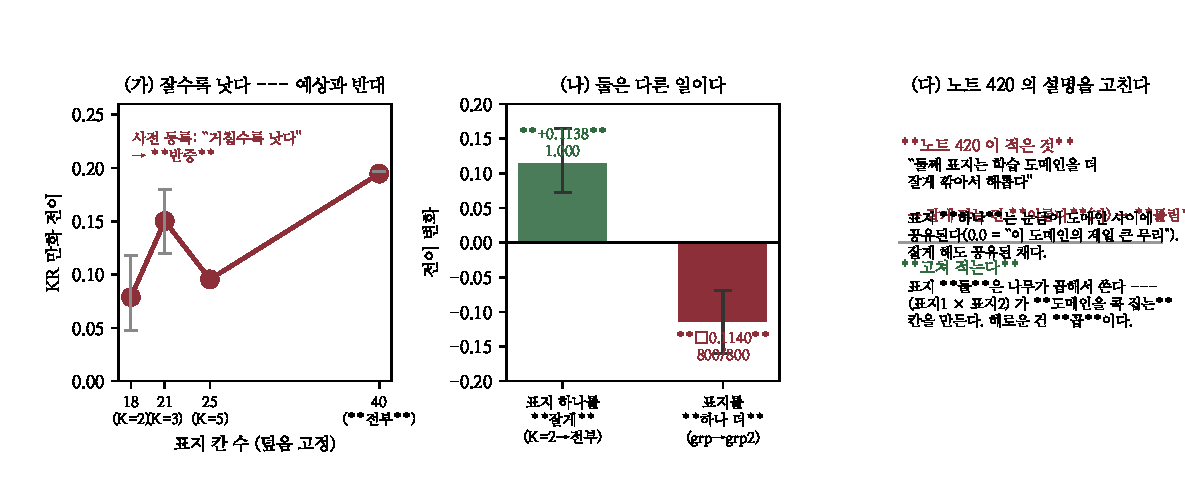
\includegraphics[width=\textwidth]{figs/fig421.pdf}
\caption{(가) 칸을 줄이면 전이가 내린다 --- 사전 등록과 반대. (나) 같은
크기, 반대 부호. (다) 노트 420의 설명을 고친다.}
\end{figure}

\end{document}
